\documentclass[11pt]{article}
\usepackage[utf8]{inputenc}
\usepackage[T1]{fontenc}
\usepackage{amsmath}
\usepackage{multicol}
\usepackage{geometry}
\usepackage{tikz}
\usetikzlibrary{shapes.geometric, arrows.meta}
\usepackage{enumitem}
\usepackage{xcolor}
\usepackage{titlesec}

% Configurações de layout
\geometry{a4paper, left=1cm, right=1cm, top=0.5cm, bottom=1.2cm}
\setlength{\columnseprule}{0.4pt}
\setlength{\baselineskip}{1.0\baselineskip}

% Cores para títulos
\titleformat{\section}{\normalfont\Large\bfseries\color{blue}}{\thesection}{1em}{}
\titleformat{\subsection}{\normalfont\large\bfseries\color{red}}{\thesubsection}{1em}{}
\titleformat{\subsubsection}{\normalfont\normalsize\bfseries\color{black}}{\thesubsubsection}{1em}{}

\title{\textcolor{blue}{Função do 2º Grau: Parábolas e Aplicações}}
\author{Professor: Jefferson}
\date{}

\begin{document}

\maketitle
\vspace{-1cm}

\begin{center}
\large{Nome: \underline{\hspace{8cm}} \quad Turma: \underline{\hspace{3cm}}}
\end{center}

\begin{multicols}{2}

\section*{1. Conceito}
Uma função do 2º grau (ou quadrática) é expressa por:
\[
f(x) = ax^2 + bx + c \quad \text{ou} \quad y = ax^2 + bx + c
\]
onde:
\begin{itemize}
    \item $a$, $b$, $c$ são coeficientes reais ($a \neq 0$)
    \item $x$ é a variável independente
    \item O gráfico é sempre uma \textbf{parábola}
\end{itemize}

\subsection*{Exemplos}
\begin{itemize}
    \item $f(x) = x^2 - 4x + 3$ \quad ($a=1$, $b=-4$, $c=3$)
    \item $y = -2x^2 + 8x$ \quad ($a=-2$, $b=8$, $c=0$)
    \item $f(x) = \frac{1}{2}x^2 + 1$ \quad ($a=\frac{1}{2}$, $b=0$, $c=1$)
\end{itemize}

\section*{2. Gráfico: Parábola}
Características principais:
\begin{itemize}
    \item \textbf{Concavidade}: Para cima ($a>0$) ou para baixo ($a<0$)
    \item \textbf{Vértice}: Ponto de máximo/mínimo
    \item \textbf{Eixo de simetria}: Linha vertical que passa pelo vértice
\end{itemize}

\begin{center}
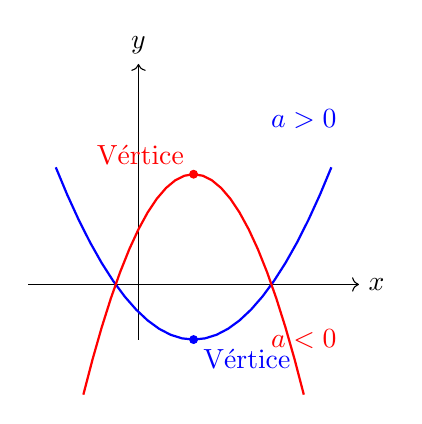
\begin{tikzpicture}[scale=0.7]
    % Eixos
    \draw[->] (-2,0) -- (4,0) node[right]{$x$};
    \draw[->] (0,-1) -- (0,4) node[above]{$y$};
    % Parábolas
    \draw[blue, thick, domain=-1.5:3.5] plot (\x, {0.5*\x*\x - \x - 0.5});
    \node[blue] at (3,3) {$a>0$};
    \draw[red, thick, domain=-1:3] plot (\x, {-\x*\x + 2*\x + 1});
    \node[red] at (3,-1) {$a<0$};
    % Vértices
    \filldraw[blue] (1,-1) circle (2pt) node[below right]{Vértice};
    \filldraw[red] (1,2) circle (2pt) node[above left]{Vértice};
\end{tikzpicture}
\end{center}

\section*{3. Concavidade}
\begin{itemize}
    \item \textbf{Para cima} ($a > 0$): Formato de "u"
    \item \textbf{Para baixo} ($a < 0$): Formato de ""
\end{itemize}

\begin{center}
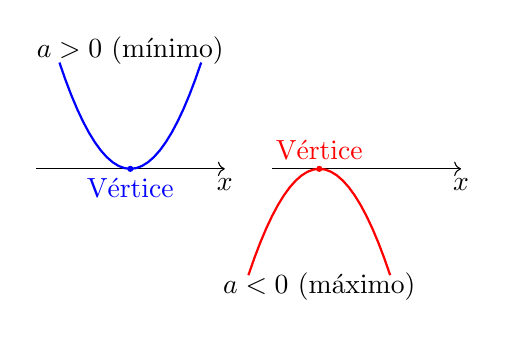
\begin{tikzpicture}[scale=0.6]
    % a > 0
    \draw[->] (-2,0) -- (2,0) node[below]{$x$};
    \draw[blue, thick, domain=-1.5:1.5] plot (\x, \x*\x);
    \filldraw[blue] (0,0) circle (1.5pt) node[below]{Vértice};
    \node at (0,2.5) {$a>0$ (mínimo)};
    % a < 0 (agora tangenciando o eixo x)
    \draw[->] (3,0) -- (7,0) node[below]{$x$};
    \draw[red, thick, domain=2.5:5.5] plot (\x, {-(\x-4)*(\x-4)}); % Equação modificada
    \filldraw[red] (4,0) circle (1.5pt) node[above]{Vértice};
    \node at (4,-2.5) {$a<0$ (máximo)};
\end{tikzpicture}
\end{center}

\section*{4. Vértice da Parábola}
Coordenadas do vértice ($V$):
\[
V\left( -\frac{b}{2a}, -\frac{\Delta}{4a} \right)
\]
onde $\Delta = b^2 - 4ac$.

\subsection*{Exemplo}
Para $f(x) = x^2 - 6x + 5$:
\[
V\left( -\frac{-6}{2\cdot1}, -\frac{16}{4\cdot1} \right) = (3, -4)
\]

\section*{5. Zeros da Função (Raízes)}
Soluções da equação $ax^2 + bx + c = 0$:
\[
x = \frac{-b \pm \sqrt{\Delta}}{2a}
\]
\begin{itemize}
    \item $\Delta > 0$: Duas raízes reais distintas
    \item $\Delta = 0$: Uma raiz real dupla
    \item $\Delta < 0$: Nenhuma raiz real
\end{itemize}

\begin{center}
\begin{tikzpicture}[scale=0.6]
    % Delta > 0
    \draw[->] (-2,0) -- (2,0);
    \draw[blue, thick, domain=-1.3:1.3] plot (\x, {\x*\x - 0.5});
    \filldraw (-0.707,0) circle (1.5pt);
    \filldraw (0.707,0) circle (1.5pt);
    \node at (0,-2) {$\Delta > 0$};
    % Delta = 0
    \draw[->] (3,0) -- (7,0);
    \draw[red, thick, domain=4.3:5.7] plot (\x, {(\x-5)*(\x-5)});
    \filldraw (5,0) circle (1.5pt);
    \node at (5,-2) {$\Delta = 0$};
    % Delta < 0
    \draw[->] (8,0) -- (12,0);
    \draw[green, thick, domain=9:11] plot (\x, {(\x-10)*(\x-10)+1});
    \node at (10,-2) {$\Delta < 0$};
\end{tikzpicture}
\end{center}

\section*{6. Estudo do Sinal}
\begin{itemize}
    \item Depende do sinal de $a$ e do $\Delta$
    \item Regra prática:
    \begin{enumerate}
        \item Identifique as raízes (se existirem)
        \item Observe a concavidade
        \item Faça o "varal" de sinais
    \end{enumerate}
\end{itemize}

\begin{center}
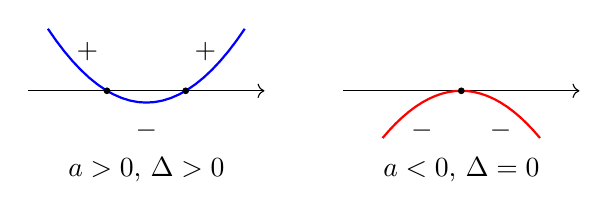
\begin{tikzpicture}[scale=0.5]
    % Caso a>0, Delta>0
    \draw[->] (-1,0) -- (5,0);
    \draw[blue, thick, domain=-0.5:4.5] plot (\x, {0.3*(\x-1)*(\x-3)});
    \filldraw (1,0) circle (2pt);
    \filldraw (3,0) circle (2pt);
    \node at (0.5,1) {$+$};
    \node at (2,-1) {$-$};
    \node at (3.5,1) {$+$};
    \node at (2,-2) {$a>0$, $\Delta>0$};
    
    % Caso a<0, Delta=0
    \draw[->] (7,0) -- (13,0);
    \draw[red, thick, domain=8:12] plot (\x, {-0.3*(\x-10)*(\x-10)});
    \filldraw (10,0) circle (2pt);
    \node at (9,-1) {$-$};
    \node at (11,-1) {$-$};
    \node at (10,-2) {$a<0$, $\Delta=0$};
\end{tikzpicture}
\end{center}

\section*{7. Aplicações Práticas}
\subsection*{Lançamento de Projétil}
A altura $h$ em função do tempo $t$:
\[
h(t) = -5t^2 + v_0t + h_0
\]
\begin{center}
\begin{tikzpicture}[scale=0.7]
    \draw[->] (0,0) -- (4,0) node[right]{$t$};
    \draw[->] (0,0) -- (0,3) node[above]{$h$};
    \draw[blue, thick, domain=0:3] plot (\x, {-\x*\x + 2*\x});
    \filldraw (1,1) circle (1.5pt) node[above right]{Vértice};
\end{tikzpicture}
\end{center}

\subsection*{Maximização de Área}
Cercar área retangular com 100m de cerca:
\[
A(x) = x(50 - x) = -x^2 + 50x
\]
Área máxima no vértice: $x = 25m$

\section*{8. Exercícios Básicos (1-10)}
\begin{enumerate}
    \item Dada $f(x) = x^2 - 5x + 6$, determine:
    \begin{enumerate}[label=\alph*)]
        \item Os coeficientes $a$, $b$, $c$
        \item As raízes
        \item O vértice
    \end{enumerate}
    
    \item Classifique a concavidade:
    \begin{enumerate}[label=\alph*)]
        \item $y = 3x^2 - 2x + 1$
        \item $f(x) = -x^2 + 4$
    \end{enumerate}
    
    \item Calcule $\Delta$ para:
    \begin{enumerate}[label=\alph*)]
        \item $x^2 - 6x + 9 = 0$
        \item $2x^2 + x - 3 = 0$
    \end{enumerate}
    
    \item Determine o vértice:
    \begin{enumerate}[label=\alph*)]
        \item $y = x^2 - 4x + 3$
        \item $f(x) = -2x^2 + 8x - 5$
    \end{enumerate}
    
    \item Esboce o gráfico de:
    \begin{enumerate}[label=\alph*)]
        \item $f(x) = x^2 - 1$
        \item $y = -x^2 + 4x$
    \end{enumerate}
\end{enumerate}

\section*{9. Exercícios Intermediários (11-20)}
\begin{enumerate}\setcounter{enumi}{5}
    \item Resolva as equações:
    \begin{enumerate}[label=\alph*)]
        \item $x^2 - 5x + 6 = 0$
        \item $2x^2 + 3x - 2 = 0$
    \end{enumerate}
    
    \item Estude o sinal:
    \begin{enumerate}[label=\alph*)]
        \item $f(x) = x^2 - 3x + 2$
        \item $y = -x^2 + 2x - 1$
    \end{enumerate}
    
    \item Aplicações:
    \begin{enumerate}[label=\alph*)]
        \item O lucro $L$ em função das unidades $x$ é $L(x) = -x^2 + 80x - 1000$. Qual o lucro máximo?
        \item Uma bola é lançada com $h(t) = -5t^2 + 20t$. Qual a altura máxima?
    \end{enumerate}
    
    \item Determine $m$ para que:
    \begin{enumerate}[label=\alph*)]
        \item $f(x) = (m-1)x^2 + 2x - 3$ tenha concavidade para cima
        \item $y = (3-m)x^2 - 4x + 1$ tenha vértice no eixo $x$
    \end{enumerate}
    
    \item Problemas:
    \begin{enumerate}[label=\alph*)]
        \item Um retângulo tem perímetro 20cm. Escreva a área em função de um lado e encontre a área máxima
        \item Qual a função quadrática que passa por (0,3), (1,4) e (2,9)?
    \end{enumerate}
\end{enumerate}

\section*{10. Exercícios Avançados (21-30)}
\begin{enumerate}\setcounter{enumi}{10}
    \item Sistemas:
    \begin{enumerate}[label=\alph*)]
        \item Resolva $\begin{cases} y = x^2 - 2x \\ y = x + 4 \end{cases}$
    \end{enumerate}
    
    \item Análise gráfica:
    \begin{enumerate}[label=\alph*)]
        \item Para $f(x) = x^2 - 4x + k$, determine $k$ para que o gráfico tangencie o eixo $x$
    \end{enumerate}
    
    \item Funções definidas:
    \begin{enumerate}[label=\alph*)]
        \item Dada $f(x) = \begin{cases} x^2, & x \leq 1 \\ 2x - 1, & x > 1 \end{cases}$, calcule $f(0)$, $f(1)$, $f(2)$
    \end{enumerate}
    
    \item Desafios:
    \begin{enumerate}[label=\alph*)]
        \item Prove que $x^2 - 2x + 1 \geq 0$ para todo $x$ real
        \item Se $f(x) = ax^2 + bx + c$ tem vértice em $(2, -1)$ e passa por $(0,3)$, determine $a$, $b$, $c$
    \end{enumerate}
    
    \item Problemas complexos:
    \begin{enumerate}[label=\alph*)]
        \item Um fazendeiro quer cercar um galinheiro retangular usando um muro como um dos lados. Se ele tem 40m de cerca, quais as dimensões para área máxima?
        \item Uma empresa estima que o custo $C(x) = 0.1x^2 - 10x + 1000$ e a receita $R(x) = 50x$. Determine o break-even point.
    \end{enumerate}
\end{enumerate}

\subsection*{Gabarito Parcial}
\begin{tabular}{|c|l|l|}
\hline
\textbf{Questão} & \textbf{Resposta} & \textbf{Questão} \\
\hline
1a) & $a=1$, $b=-5$, $c=6$ & 16a) & $m>1$ \\
1b) & $x=2$ e $x=3$ & 16b) & $m=7$ \\
1c) & $V(2.5, -0.25)$ & 17a) & $(4,8)$ e $(-1,3)$ \\
2a) & Concavidade para cima & 18a) & $k=4$ \\
2b) & Concavidade para baixo & 19a) & $0$, $1$, $3$ \\
3a) & $\Delta = 0$ & 20a) & $10m \times 20m$ \\
3b) & $\Delta = 25$ & 20b) & $x \approx 22$ ou $x \approx 45$ \\
\hline
\end{tabular}

\end{multicols}

\end{document}
